\documentclass[12pt]{article}
\usepackage{longtable}
\usepackage{makecell}
\usepackage{float}
\usepackage{graphicx}
\usepackage{bm}
\usepackage{placeins}
\usepackage{booktabs}
\usepackage{gensymb}
\usepackage{amssymb}
\usepackage{indentfirst}
\usepackage{threeparttable} 
\usepackage{multirow}
\usepackage{aligned-overset}
\usepackage[slantfont,boldfont]{xeCJK}
\usepackage{fontspec}
\renewcommand{\arraystretch}{1.5}
\usepackage[paperwidth=23cm,paperheight=37.21cm]{geometry}
\setCJKmainfont{SimSun}
\setmainfont{SimSun}
\setsansfont{SimSun}
% 设置正文字体为四号（12pt）
% \renewcommand{\CJKmainfont}{SimSun}
\renewcommand{\CJKfamilydefault}{\CJKrmdefault}
\renewcommand{\normalsize}{\fontsize{12pt}{18pt}\selectfont}
\normalsize

\title{粘滞现象2实验报告}
\author{2411545 邱凯锐}
\date{2025.10.17}

\begin{document}
\maketitle
\section{实验背景}
\subsection{理论知识}
由于空气的粘性作用，物体表面会产生与物面相切的摩擦力，全部摩擦力的合力称为摩擦阻力。
与物面垂直的气流压力合成的阻力称为压差阻力。
在实际流体中，粘性作用下不仅会产生摩擦阻力，而且会使物体后方气流压强分布有别于理想流体中的分布情况，
并产生压差阻力，两种阻力常同时存在。
以流体绕过某物体的流动为例，两种阻力的相对大小取决于下列三个因素：

\begin{enumerate}
  \item 物体的形状：如果物体是球那样的钝体，边界层分离较早，压差阻力是主要的；
        对于流线型物体，边界层不分离或分离较迟，则压差阻力较小，摩擦阻力是主要的。
  \item 物体特征长度决定的雷诺数的大小。雷诺数决定边界层中的流动状态。
        层流边界层摩擦阻力较大，但因分离推迟，往往压差阻力较小；
        层流则相反，摩擦阻力较小，而压差阻力较大。
  \item 物体表面的粗糙度。粗糙表面的摩擦阻力较大，但粗糙表面可促进边界层湍化，
        使分离推迟，从而减小压差阻力。
\end{enumerate}

\textbf{曳力系数（drag coefficient）}
又称流体阻力系数，是指一个物体在流体（液体或气体）中和流体有相对运动时，
物体会受到流体的阻力。牛顿是已知的第一个在实验中测量出大概定性的曳力系数的科学家。
他测量了从 Saint Paul’s Cathedral 的圆顶掉落的小球的速度，得到了 1000 到 2000 范围的雷诺数。
他将自己的数据用经验公式的形式表示为：

\begin{equation}
U_t^2 = \frac{3 D_p (\rho_s - \rho_f) g}{\rho_f C_d}
\end{equation}
其中，球体的曳力系数约为：
\[
C_d = 0.44
\]

阻力的方向和物体相对于流体的速度方向相反，其大小和相对湿度的大小有关。在相对速率 $v$ 较小时，阻力 $f$ 的大小与 $v$ 成正比：$f=kv$ （比例系数 $k$ 决定于物体的大小和形状以及流体的性质）；在相对速率较大以至于物体的后方出现流体漩涡时，阻力表示为
\begin{equation}
    f=\frac 12C_D\rho_A Av^2
\end{equation}
其中 $\rho_A$ 是空气密度，$A$ 是物体的有效横截面积，$C_D$ 为曳力系数。曳力系数 $C_D$ 的大小取决于物体形状和雷诺数。

\textbf{雷诺数（Reynolds number）}，是流体力学中表征粘度影响的相似准测数，记作 $Re$ 。雷诺数的意义是流体的惯性力与粘性力之比。既然惯性力其实就是流体运动状态的改变（加速度），那么雷诺数其实就代表了流动时粘性力的大小。
\begin{equation}
    Re=\frac{\rho_AvD_B}{\mu_A}
\end{equation}
其中 $v$、$\rho_A$、$\mu_A$ 分别为流体的速度、密度和动力粘滞系数， $D_B$ 为特征长度。利用雷诺数可区分流体的流动时层流或湍流，也可用来确定物体在流体中流动所受到的阻力。雷诺数从小到大的变化就是粘性力逐渐减弱的过程。

\subsection{风洞}
如 Figure 1，密度为 $\rho_A$，速度为 $v_0$ 的空气流过截面积为 $A_0$ 的管道，风流具有的功率为
\begin{equation}
    P_W=\frac 12\rho_AA_0v_0^3
\end{equation}

\begin{figure}[h]
    \centering
    
\includegraphics[width=0.8\textwidth]{fig1.png}
    \caption{管状风流（横截面积为 $A_0$）}
\end{figure}

本实验采用计算机风扇作为风发生器将风洞中的风吸出（排风型风扇），以获得平缓的气流，风洞装置实物如 Figure 2 所示。使用简单的光传感电路（如 Figure 3 所示）来测量涡轮扇叶的转动频率；光电传感器含有 1 对红外发射器和接收器，涡轮扇叶上贴有反光片，扇叶转动时可探测到该反光片发出的反射光，用示波器测量光传感器接收到的反射光信号（风扇转动频率）。

\begin{figure}[h]
    \centering
    
\includegraphics[width=0.8\textwidth]{fig2.png}
    \caption{风洞装置实物图}
\end{figure}

\begin{figure}[h]
    \centering
    
\includegraphics[width=0.8\textwidth]{fig3.png}
    \caption{工作电路图}
\end{figure}

风洞内风速主要取决于风发生器（计算机风扇）电机的转动频率 $f_M$ ，一般来说具有线性关系，在本次实验中会对此进行测量和拟合。

\subsection{风速的测量}
本实验采用热线式风速仪对风速进行测量。注意实验中风速仪的热丝应在欲测量风速的位置（即风洞中心）

我们还可以通过乒乓球摆来设计一个测量风速的简单方法。如 Figure 4 所示，风会给乒乓球一个拉力，使乒乓球摆偏斜一个角度 $\theta$ ，这个拉力表达式为
\begin{equation}
    F_D=\frac 12C_D\rho_AA_Bv^2
\end{equation}
其中 $C_D$ 使物体的拉力系数，$\rho_A$ 是空气的密度，$A_B$ 是乒乓球的横截面积，$v$ 是乒乓球相对于空气的速度。

\begin{figure}[h]
    \centering
    
\includegraphics[width=0.8\textwidth]{fig4.png}
    \caption{(a) 乒乓球风速计示意图，(b) 实验装置，(c) 乒乓球，(d) 风洞外侧的读数刻度尺}
\end{figure}

\section{实验装置}
1.贴有刻度尺的风洞 2.计算机风扇:带有光电传感器 3.系有细线的小球 4.示波器:用于频率测量 5.刻度尺(50cm)6.固定支架，铁架台 7.游标卡尺8.电子天平 9.导线若干根 10.双通道电源 11.热线式风速仪

\begin{figure}[h]
    \centering
    
\includegraphics[width=0.7\textwidth]{1.jpg}
    \caption{实验装置}
\end{figure}

\section{实验步骤}

1. 如 Figure 3 所示连接光电传感器电路，打开电源开关使风扇转动，调节电源电压大小可以控制风扇转动频率，示波器读出风扇转动频率 \( f \) 的大小，使用风速仪测量风洞中心位置的风速，以表格形式记录数据，并绘制关系曲线，通过拟合得到风速 \( v \) 与转动频率 \( f \) 的关系表达式。

2. 如 Figure 4（b）所示，将摆线塞进印有刻度尺的狭缝中，将乒乓球放置在风洞管道的中心。风扇打开时，小球在风的作用下会偏向一边，假设此时丝线与竖直方向夹角为 \( \theta \)。画出乒乓球受力图。根据公式（5），利用函数变换，推导出风速 \( v \) 和偏移角 \( \theta \) 的函数关系。（函数关系式中空气质量密度 \( \rho_A \) 和乒乓球质量 \( m_B \) 以及其他的一些参量作为已知量或直接测量量。刻度尺用于计算偏移角 \( \theta \)。）

3. 改变风速，测量乒乓球偏移角 \( \theta \)，以表格形式记录实验数据。计算不同风速下的曳力系数 \( C_D \) 及雷诺数 \( Re \)。画出雷诺数与曳力系数的关系曲线。

4. 球面的曳力系数随雷诺数的变化关系如 Figure 6 所示。根据你得出的曳力系数 \( C_D \) 和雷诺数 \( Re \) 的关系曲线，在图上画出（标出）属于哪个区间段，并对实验结果进行分析。

5. 改变球的直径或选择表面粗糙度不同的球，继续进行实验探究，重复 2、3、4 步。

\begin{figure}
    \centering
    
\includegraphics[width=0.6\textwidth]{fig5.png}
    \caption{球面的曳力系数随雷诺数的变化关系图}
\end{figure}

\section{实验数据}
1. 风速 $v$ 与转动频率 $f$ 的测量数据

\begin{table}[H]
    \centering
    \caption{$v-f$ 测量数据}
    \vspace{2pt}
    \begin{tabular}{ccccccc}
        \hline \hline
        v(m/s) & 0.51 & 0.66  & 1.1   & 1.47  & 1.76  & 2.02  \\
        f(Hz)  & 7.85 & 10.58 & 15.63 & 20.05 & 24.04 & 27.62 \\ \hline
        v(m/s) & 2.24  & 2.48  & 2.71  & 2.87  & 3.06  & 3.28 \\
        f(Hz)  & 30.86 & 33.94 & 36.76 & 39.47 & 41.67 & 43.86 \\ \hline \hline
    \end{tabular}
\end{table}
经过线性拟合得到 Figure 5,以及 $v-f$ 关系：
\begin{equation}
    v=0.0762f-0.0967
\end{equation}

\begin{figure}[H]
    \centering
    
\includegraphics[width=0.6\textwidth]{Figure_1.png}
    \caption{ $v-f$ 拟合曲线}
\end{figure}

2. 根据受力平衡（受力示意图如 Figure 6）
\begin{equation}
    F_D=mg \tan \theta
\end{equation}
得到
\begin{equation}
    v=\sqrt{\frac{2mg\tan \theta}{C_D\rho_AA_B}}
\end{equation}

\begin{figure}[h]
    \centering
    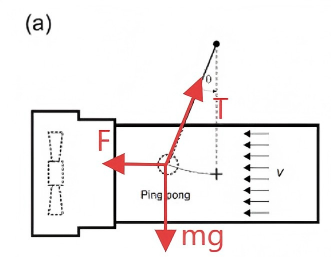
\includegraphics[width=0.4\textwidth]{fig4(1).png}
    \caption{小球受力示意图}
\end{figure}

3.小球 $\theta-v$ 实验数据 

\begin{table}[H]
    \centering
    \caption{乒乓球 $\theta-v$ 实验数据}
    \vspace{2pt}
    \begin{minipage}{0.7\textwidth}
        \raggedleft
        $h=16\ \mathrm{cm}$，$m=2.768\ \mathrm g$，$d=4.010\ \mathrm{cm}$ 
    \end{minipage}\\[2pt]
    \begin{tabular}{ccccccc}
        \hline \hline
        $f(\mathrm{Hz})$  & 7.25  & 9.85  & 14.79 & 19.23 & 23.15 & 26.88 \\
        $v(\mathrm{m/s})$ & 0.46  & 0.65  & 1.03  & 1.37  & 1.67  & 1.95  \\
        $\Delta s(\mathrm{cm})$ & 0.1   & 0.2   & 0.25  & 0.4   & 0.55  & 0.8   \\
        $\theta$      & 0.006 & 0.012 & 0.016 & 0.025 & 0.034 & 0.050 \\
        \hline
        $f(\mathrm{Hz})$  & 30.34 & 33.56 & 36.59 & 39.27 & 41.84 & 44.25 \\
        $v(\mathrm{m/s})$ & 2.22  & 2.46  & 2.69  & 2.90  & 3.09  & 3.28  \\
        $\Delta s(\mathrm{cm})$ & 1     & 1.2   & 1.3   & 1.5   & 1.7   & 2.2   \\
        $\theta$      & 0.062 & 0.075 & 0.081 & 0.093 & 0.106 & 0.137 \\
        \hline \hline
    \end{tabular}
\end{table}

\begin{table}[H]
    \centering
    \caption{粗糙小球 $\theta-v$ 实验数据}
    \vspace{2pt}
    \begin{minipage}{0.7\textwidth}
        \raggedleft
        $h=17\ \mathrm{cm}$，$m=3.134\ \mathrm g$，$d=3.608\ \mathrm{cm}$ 
    \end{minipage}\\[2pt]
    \begin{tabular}{ccccccc}
        \hline\hline
        $f(\mathrm{Hz})$  & 7.85  & 10.58 & 15.63 & 20.05 & 24.04 & 27.65 \\
        $v(\mathrm{m/s})$ & 0.50  & 0.71  & 1.09  & 1.43  & 1.74  & 2.01  \\
        $\Delta s(\mathrm{cm})$ & 0.05  & 0.9   & 0.2   & 0.3   & 0.45  & 0.6   \\
        $\theta$      & 0.003 & 0.053 & 0.012 & 0.018 & 0.026 & 0.035 \\
        \hline
        $f(\mathrm{Hz})$    & 31.06 & 34.25 & 37.04 & 39.68 & 42.02 & 44.44 \\
        $v(\mathrm{m/s})$    & 2.27  & 2.51  & 2.73  & 2.93  & 3.11  & 3.29  \\
        $\Delta s(\mathrm{cm})$    & 0.8   & 1     & 1.2   & 1.4   & 1.5   & 1.7   \\
        $\theta$    & 0.047 & 0.059 & 0.070 & 0.082 & 0.088 & 0.100 \\
        \hline \hline
    \end{tabular}
\end{table}

\begin{figure}[H]
    \centering
    
\includegraphics[width=0.8\textwidth]{Figure_2.png}
    \caption{曳力系数随雷诺数的变化关系图}
\end{figure}

\end{document}